\documentclass[14pt, oneside]{memoir}

\usepackage{amsmath}
\usepackage{graphicx} %for image inclusion
\usepackage{float} %for image placement
\usepackage{listings} %for code inclusion
\usepackage{color} %for code color
%\usepackage{fontspec}

%\setmainfont[Ligatures=TeX]{Segoe Print}
%\setmainfont[Ligatures=TeX]{Comic Sans}

\usepackage{kantlipsum}

\usepackage{duck}

\lstdefinestyle{customarduino}{belowcaptionskip = 1\baselineskip,
breaklines = true,
frame = L,
xleftmargin=\parindent,
language=C,
showstringspaces=false,
basicstyle=\footnotesize\ttfamily,
keywordstyle=\bfseries\color{green!40!black},
commentstyle=\itshape\color{purple!40!black},
identifierstyle=\color{blue},
stringstyle=\color{orange},
}

\begin{document}



\title{\textbf{NAILAB ARDUINO BOOTCAMP}}
\author{John Nduli and Christopher Bartonjo} 
 \maketitle


\chapterstyle{weloveducks}

\setlength{\parskip}{1.5\baselineskip}
\setlength{\parindent}{0pt}
%\OnehalfSpacing{}
\chapter{The journey begins}
Hi, I am a duck. Quack! You'll see me a lot. I'll guide you
through the notes. Also, I hope you can see the flowers above,
they're there to show your progress. `Yaaaah!'

\section*{Introduction}
Voltage is the potential energy between two points in a circuit.
\\
Current is the rate of flow of charge in a circuit.
\\
Image a tank with water. Voltage is similar to the pressure in the
tank. The larger the tank, the more the pressure.
\\
Current is the rate of flow of the water when the tap is opened.
The larger the tank, the faster the water flows.
\\
Resistance is the tap. If is opened completely (similar to lower
resistance), the water will flow faster. If opened about halfway,
the water will flow slowly.
\\
The following equations will help you out a lot:
\begin{align}
    V &= I * R \\
    I &= \frac{V}{R}\\
    R &= \frac{V}{I}
\end{align}
\section*{LEDs}
LED is an electronic device that produces light when voltage and
current is supplied through it.
\\
It is stands for Light Emitting Diode.
\\
The following schematics show how to connect LEDs.
\begin{figure}[h]
    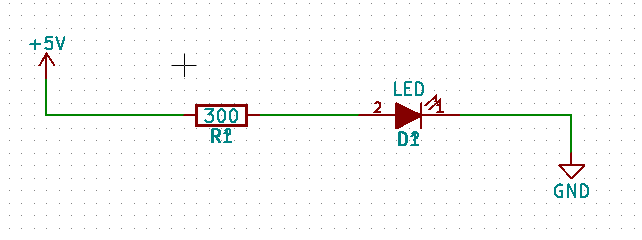
\includegraphics[width=\linewidth]{circuit_images/one_led.png}
    \caption{one led in a circuit}
\end{figure}
\begin{figure}[H]
    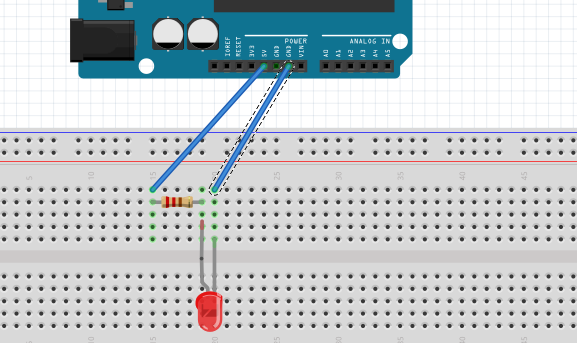
\includegraphics[width=0.7\linewidth]{./circuit_images/fritz_one_led.png}
    \caption{One LED in a circuit set up on breadboard}
\end{figure}

\begin{figure}[H]
    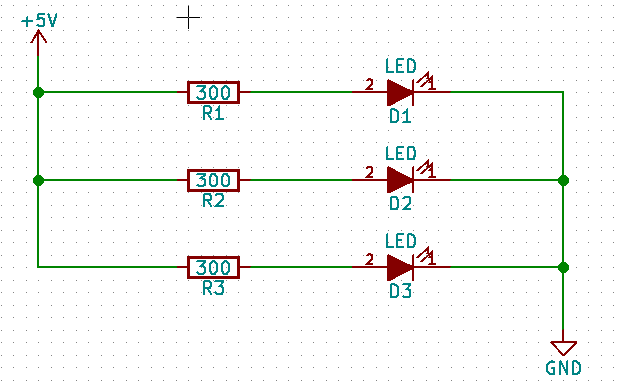
\includegraphics[width=0.7\linewidth]{circuit_images/multiple_leds.png}
    \caption{Multiple LEDs in a circuit}
\end{figure}

\section*{Programming LEDS}
Similar to the ciruits made in the previous section. However,
instead of directly supplying 5V to the LEDs, we will use the
arduinos Input Output pins to supply the power.
\\
For example make a circuit similar to the one led circuit. The
wire that comes from the 5V of the arduino, now place it in the
hole labelled 1 on the arduino.
\\
Then open the arduino software and write the following code:
\lstinputlisting[caption=blinkingled,
style=customarduino]{../codes/ledblink/ledblink.ino}

For multiple LEDs connect the circuit as shown below:
\begin{figure}[H]
    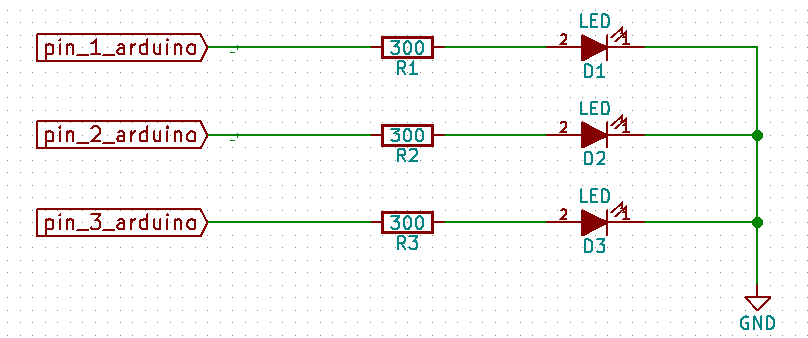
\includegraphics[width=\linewidth]{circuit_images/blinking_leds.png}
    \caption{Blinking LEDs in a circuit}
\end{figure}

Here is the code for the arduino:

\lstinputlisting[caption=Three Blinking LEDs,
style=customarduino]{../codes/threeleds/threeleds.ino}

And here is how the circuit should look like:
\begin{figure}[H]
    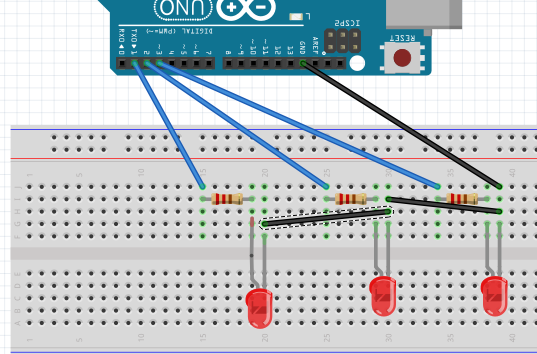
\includegraphics[width=0.7\linewidth]{circuit_images/fritz_blinking_leds.png}
    \caption{Blinking LEDs in a breadboard}
\end{figure}

\chapter{More about LEDs}
So we've made it to the next part. Yaah. This is a really
interesting section. We'll learn about sensors and use a buzzer.

\section*{RGB LED}
The RGB LED is different from the LEDs seen so far. It contains
four legs, three of the same size and one really long one.
\\
It also has three different colors: Reg, Green and Blue.
\\
If you connect the longest pin to ground and place resistors on
each of the other legs similar to the circuits made in the LED
section, that is assume each leg is the longest leg of a 2 pin
resistor, then provide 5V to each leg, you will see the different
colors.
\\
\begin{figure}[H]
    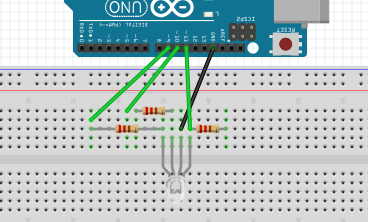
\includegraphics[width=\linewidth]{circuit_images/rgb_led.png}
    \caption{RGB LED in a circuit}
\end{figure}

The following is the code used:
\lstinputlisting[caption=BlinkingLED,
style=customarduino]{../codes/rgbled/rgbled.ino}


\section*{Infra Red LEDs}
The IR transmitter is a special LED that transmits Infra Red. Wheh
connected, the light cannot be seen by a naked eyq. However some
phone cameras can see the light (it will have a pink color).
\\
The IR receiver (black LED) is used to detect the presence of
InfraRed.
It produces a voltage in response to the same.

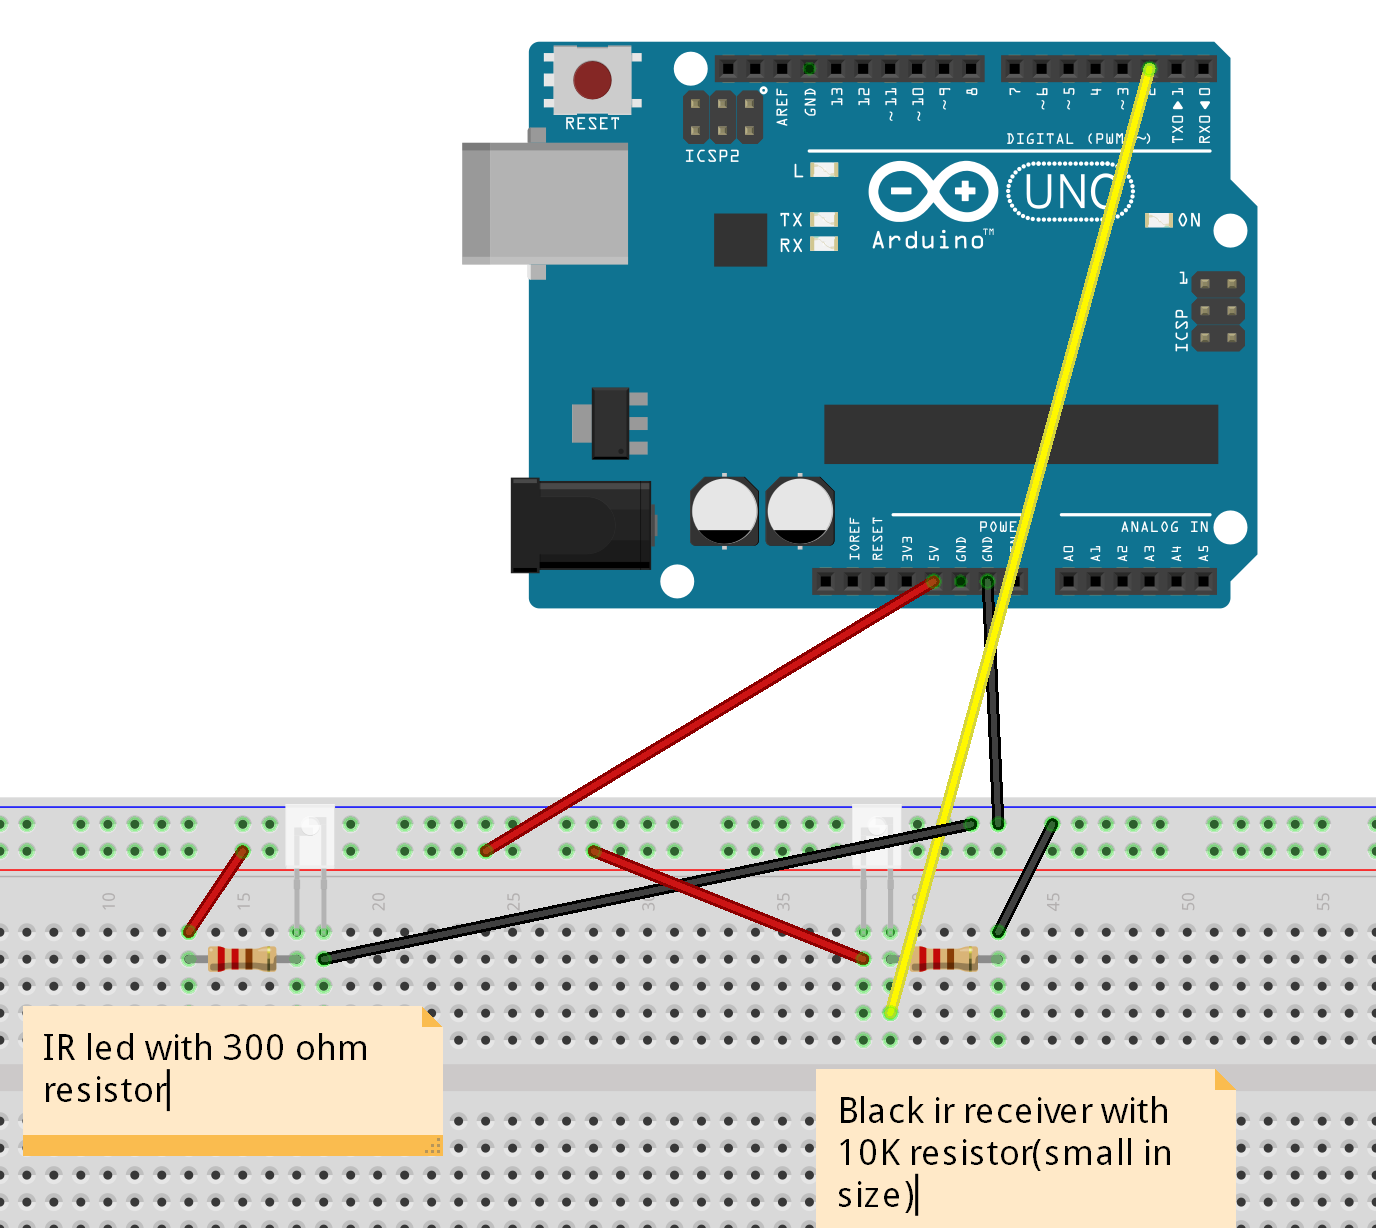
\includegraphics[width=7.06667in,height=4.58788in]{circuit_images/ir_circuit.png}

From the diagram above, the red wire is connected to the 5v power
supply, 
then the IR led long leg is connected to the 5v through the 300
Ohm
resistor, the short leg is connected to ground (the black wire is the
ground connection).
\\
The black IR (not black in the diagram) is connected to the 5v power
supply on the short leg. A 10K resistor (remember that the 10K resistor
is the small cream-colored resistor) is connected to the long leg and
the other end of the 10K resistor is connected to ground. The black wire
is the ground connection.

The yellow wire is connected to the long leg of the black IR led and the
other end connected to pin 2 of the Arduino.

That's it!

Run the following code to confirm your circuit:

\lstinputlisting[caption=IR Sensor,
style=customarduino]{../codes/irsensor/irsensor.ino}


\begin{itemize}
    \item Since we are reading the signal from pin 2, we set it as
        input to the Arduino to read from it.
    \item Serial.begin(9600) starts the serial monitor so that we
        can use it to see if our program is running well.
    \item When we obstruct the IR led, we should read ``\emph{Stop
        Blocking me!}'' in the serial monitor
    \item When there is no obstruction we should read ``\emph{I
        can see my light but not you!}''. Try and figure out that quote ; ).
    \item digitalRead(2) means we are instructing Arduino to read
        pin 2 for data. If there is no obstruction, we expect a 1
        but when we block the IR we should get a 0.
\end{itemize}


\section*{Buzzer}
The buzzer is almost like a small speaker.
\\
When a changing voltage is applied to it, it will produce sound or
a tone.
\\
The arduino software has an example that runs of the buzzer.
\\
To access this, go to `File' -$>$ `Examples' -$>$ `Digital' -$>$
`toneMelody'
\\
Here is the circuit that works with the given example:
\begin{figure}[H]
    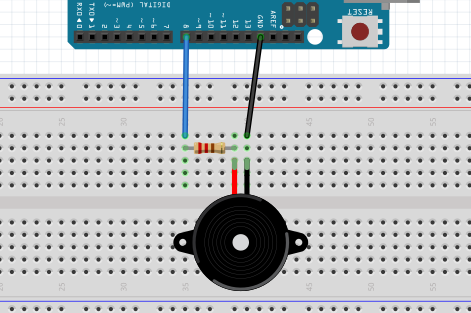
\includegraphics[width=0.7\linewidth]{circuit_images/buzzer.png}
    \caption{Buzzer circuit}
\end{figure}

You can play with the tunes and timings to get unique music
compositions.

\chapter{Now what}
It's feels as though we've learned so much in so little time. What
else can we learn?

\section*{Servo Motor}
A servo motor is a motor that can be precisely controlled.\\
\begin{figure}[h]
    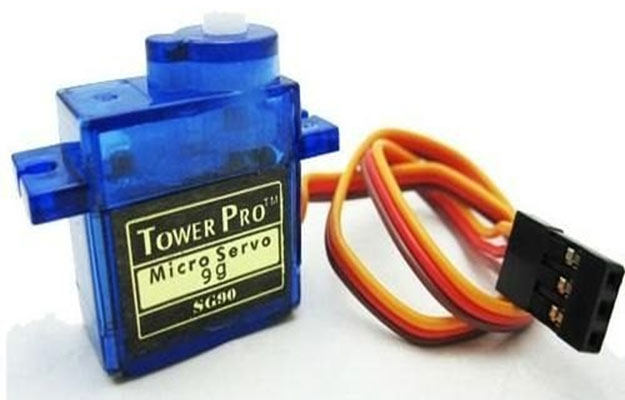
\includegraphics[width=0.5\linewidth]{./circuit_images/servo_motor.jpg}
    \caption{Servo Motor}
\end{figure}

To connect the servo, it should have three differenly coloured
wired:
\begin{enumerate}
    \item Red: this goes to 5V
    \item Orange: this goes to a PWM pin, that is a pin with
        '$\sim$' sign on it.
    \item Brown or Black: this goes to GND
\end{enumerate}

The arduino software has an example that runs of the servo.
\\
To access this, go to `File' -$>$ `Examples' -$>$ `Servo' -$>$
`sweep'
\section*{DC Motor}
A dc motor is a motor that can be driven by dc voltage, for
example a battery
\\
Mostly a driver is used to control the on and off of the dc motor.
The L298 driver was used in this class.
\\
From the underside of the L298 driver shield (Red board), there is
IN1, IN2, IN3, and IN4. These will be the inputs from the arduino.
\\
Also there are GND, +12V, +5V, which are where the voltage sources
are connected.
\\
Then there are OUT1, OUT2, OUT3 and OUT 4, from which the motors
are connected.
\\
The circuit is shown below:

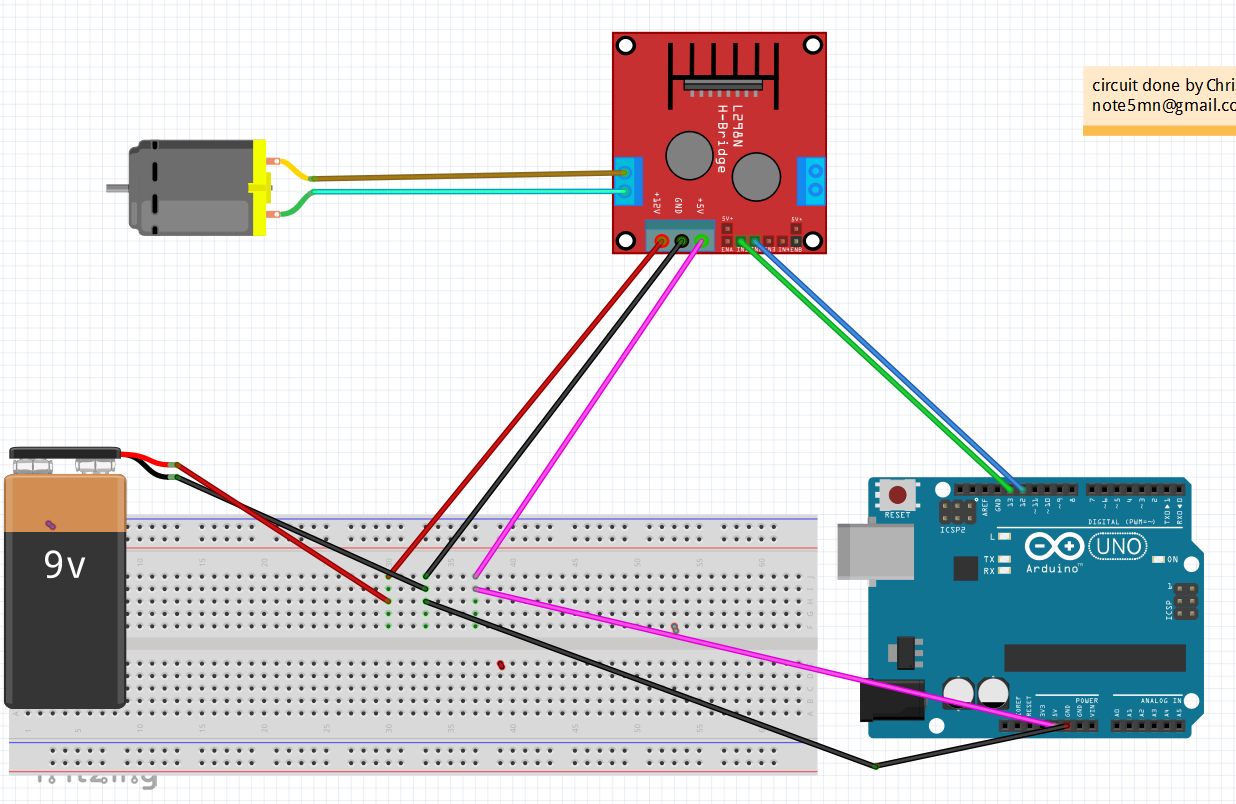
\includegraphics[width=6.49091in,height=3.82013in]{circuit_images/dc_motor_driver.png}

From the circuit above, we require the following components:
\begin{itemize}
    \item Arduino
    \item L298 Motor Driver
    \item 1 dc motor
    \item 9V battery with terminals
    \item Breadboard
    \item wires
\end{itemize}
Connect the ground of the driver, ground of Arduino and the black wire
of the battery on the same rail on the breadboard as shown.
\\
Connect the red wire of the batter to the terminal block labeled +12v on
the motor driver.
\\
Connect pins 12 and 13 to header pins labeled IN1 and IN2 on the motor
driver.
\\
Connect the motor pins to terminal block written OUT1 and OUT2.

\lstinputlisting[caption=DC Motor with L298,
style=customarduino]{../codes/dc_motor_driver/dc_motor_driver.ino}


Run the above code and observe what is happening.

We set pin12 and pin13 as outputs so that we can write to these pins

Writing a pin high causes the motor to rotate in one direction and
writing a pin low causes the motor to stop.

\section*{Bluetooth}

Bluetooth is a means of communication between two or more devices.
Locally it is mainly used in phone to transfer files.
\\

To use bluetooth with the arduino we will need:
\begin{enumerate}
        \def\labelenumi{\arabic{enumi}.}
    \item
        Bluetooth module
    \item
        2 LEDs
    \item
        Arduino
    \item
        300 ohm resistors
\end{enumerate}

The following is the ciruit:

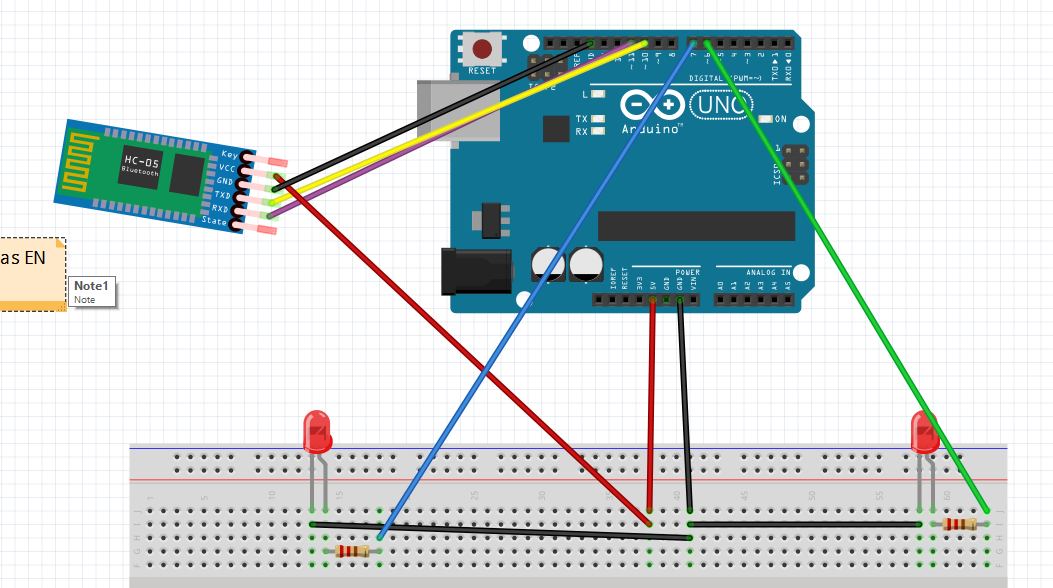
\includegraphics[width=6.89091in,height=3.81659in]{circuit_images/bluetooth.png}


Connect the circuit as shown above. The TX from the Bluetooth goes to
pin10 of the Arduino. The RX from the Bluetooth goes to pin11 of the
Arduino.
\\
Remember that when connecting the LEDs, the 5v connects to the long leg
through the 300ohm resistor. Also, the short leg is connected to the
ground.

\lstinputlisting[caption=blinkingled,
style=customarduino]{../codes/bluetooth/bluetooth.ino}

\chapter{What Next}

With what you have learnt, you can build and make a large variety
of interesting projects.

To help you out, we have compiled a small list of projects that
can be made:
\begin{description}
    \item [Bluetooth controlled car]: This will combine your
        knowledge of bluetooth and DC motors. To rotate corners,
        you can lower the speed of one side of the motor.
    \item [Robotic arm]: This will combine your knowledge of
        servos and the arduino. The make it more interesting, you
        can add bluetooth to control the arm.
    \item [Burglar alarm system] This will combine the IR
        transmitter and receiver for the burglar detection, the
        buzzer for an alarm system and LEDs for signals.
    \item [LED light signs] This can vary greatly. You can try to
        implement the traffic lights of a product light, for
        example the Mpesa signs. You can also go for a completely
        unique pattern.
    \item [Room Air Conditioner]: This combines the knowledge of
        the temperature sensor and the dc motor.

\end{description}

\end{document}
